%!TEX root = ../main.tex

\graphicspath{{./figures/introduction/}}

\chapter{FISH-based transcriptomics}
\label{ch:introduction}

\minitoc
\newpage

%%%%%%%%%%%%%%%%%%%%%%%%%%%%%%%%%%%%%%%%%%%%%%%%%%%%%%%%%%%%%%%%%%%%%%%%%%%%%%%%%%%%%%%%%%%%%%%%%%%%%%%%%%%%%%%%%%%%%%%%%%%%%%%%%%%%%%%%%%%%%%%%%%%%%%%%%%%%
%%%%%%%%%%%%%%%%%%%%%%%%%%%%%%%%%%%%%%%%%%%%%%%%%%%%%%%%%%%%%%%%%%%%%%%%%%%%%%%%%%%%%%%%%%%%%%%%%%%%%%%%%%%%%%%%%%%%%%%%%%%%%%%%%%%%%%%%%%%%%%%%%%%%%%%%%%%%
%%%%%%%%%%%%%%%%%%%%%%%%%%%%%%%%%%%%%%%%%%%%%%%%%%%%%%%%%%%%%%%%%%%%%%%%%%%%%%%%%%%%%%%%%%%%%%%%%%%%%%%%%%%%%%%%%%%%%%%%%%%%%%%%%%%%%%%%%%%%%%%%%%%%%%%%%%%%

\section{Gene expression process}
\label{sec:gene_expression}

Cells are the basic unit of all living organisms.
Yet, a diversity of cell-type exists, performing different actions.
Some of those are common among all cells (cell division for example), but others can be very specific.
Most of the time, different cell-types perform diverse actions through a different set of functional molecules.
In order to implement these different cellular processes and to fulfill the variety of diverse functions, a cell gets its instructions from the \ac{DNA}.
The latter contains all the cell's genetic information and it is common for all cells of the same organism.
A \ac{DNA} strand presents a succession of genes, defined as long sequences of nucleotides.
They are organics molecules composed of a five-carbon sugar, a phosphate group and one of the four nucleobases: Adenine, Cytosine, Guanine and Thymine.
Together, these nucleobases form a genetic alphabet of 4 letters (A, C, G and  T).
Each gene encodes the blueprint of a functional molecule with a specific sequence of nucleobases.

Gene expression is the process by which genetic information is transformed into functional products.
\ac{RNA} molecules, or transcripts, are essential for this process.
They are either the functional gene products themselves or they serve as an intermediate molecule prior to the production of other functional products, namely the proteins.
A change in gene expression gives cells enough flexibility to adapt and react to different external stimuli.
It also drives cells differentiation, allows them to run their basic functions, modulate their activities and therefore appears to be one of the most fundamental processes of life.
On the contrary, its deregulation can lead to various diseases.
This explains the interest of the scientific community to study and decode gene expression processes.

\begin{figure}[h]
    \centering
    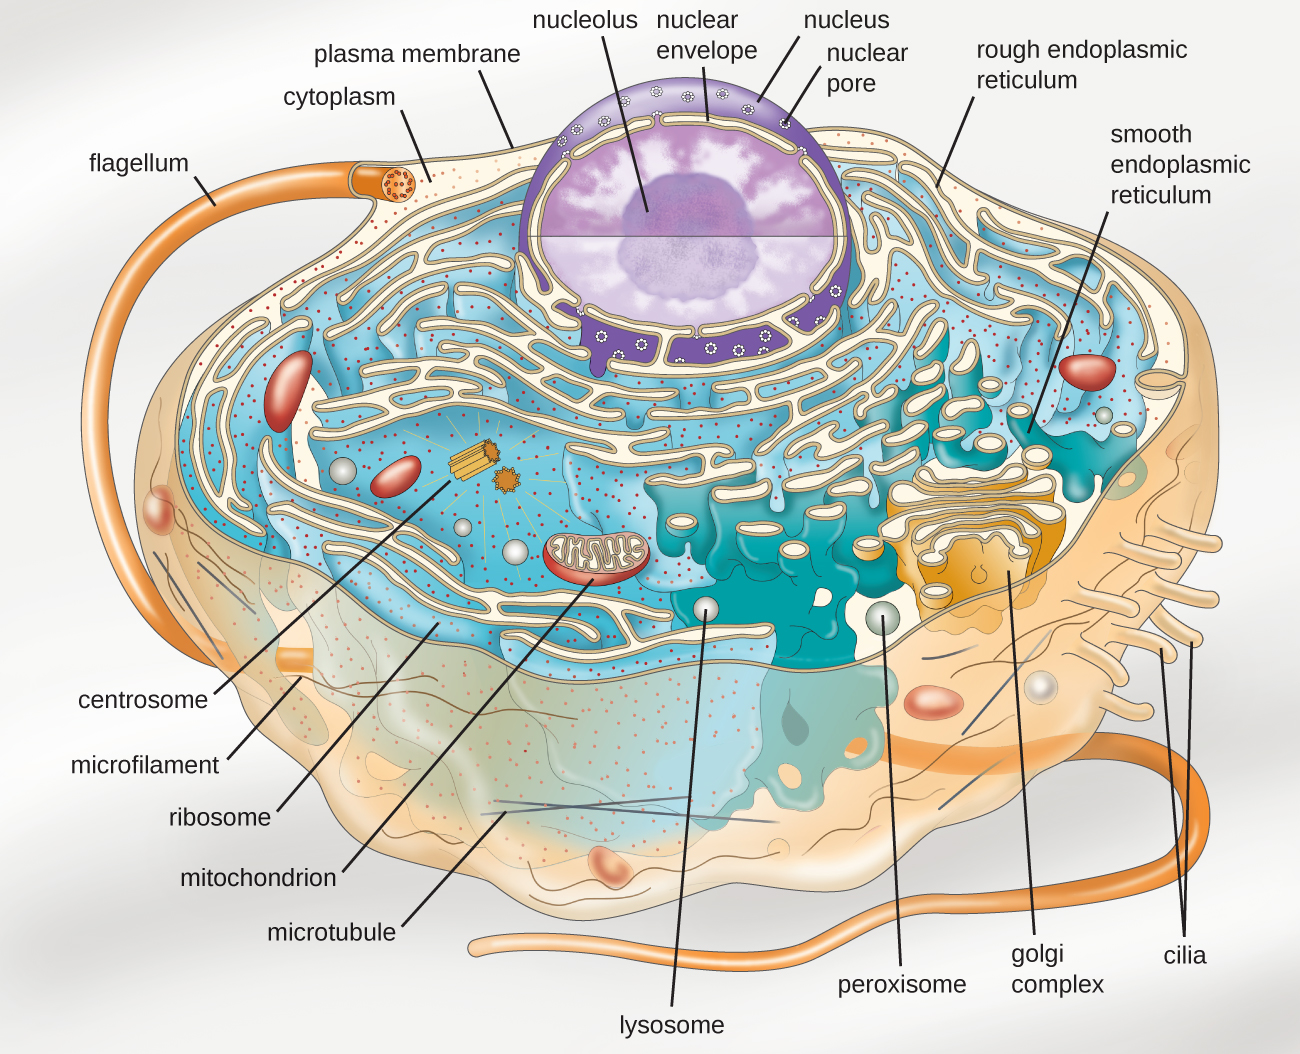
\includegraphics[width=0.8\textwidth]{figures/introduction/cell_eukaryotic.jpg}
    \caption[Eukariotic cell]{Illustration of an eukaryotic cell, from~\cite{parker2017microbiology}}
    \label{fig:eukaryotic_cell}
\end{figure}

In the living world, cells can be divided in two categories: prokaryotic cells and eukaryotic cells.
The prokaryotic cells, which do not have a nucleus and typically form a unicellular organism, and the eukaryotic cells, with a well-organized nucleus.
An eukaryote (a living organism with eukaryotic cells) is usually composed of cells with a higher level of compartmentalization through membrane-bound organelles.
The nucleus is obviously the most important of these organelles, with the \ac{DNA} inside.
The rest of the organelles are located in the cytoplasm, such as the mitochondria, the lysosomes, or the Golgi apparatus (see Figure~\ref{fig:eukaryotic_cell}).

For an eukaryote cell, the expression of a gene includes two main steps: the transcription of a \ac{DNA} sequence into a \ac{RNA} (in the nucleus) and the translation of a \ac{RNA} into a protein.
Between these two major steps, there is a phase of maturation for the transcript, before a potential exports outside the nucleus and a transport somewhere in the cytoplasm.
A cell can regulate either the transcription or the translation step to control the production of its functional molecules and thereby the biological process to which the proteins or \ac{RNA} contribute.

\subsection{Transcription}
\label{subsec:intro_transcription}

\subsubsection{The primary transcripts}

This step consists in copying a gene (a sequence of nucleotides along the \ac{DNA} strands) into another biomolecules composed of nucleotides: a \ac{RNA}.
While the \ac{DNA} is stuck within the nucleus, the \ac{RNA} can convey the blueprint of the future protein outside.
In many cases, \ac{RNA} can be non-coding (they do not lead to the synthesis of a protein) and fulfill a variety of functions itself, for instance the regulation of gene expression.
In a \ac{RNA}, the nucleotide Uracil (U) replaces the Thymine (T) and a ribose sugar serves as backbone instead of a desoxyribose sugar.
If both \ac{DNA} and \ac{RNA} contain genetic information, \ac{RNA} is a shorter single-stranded molecule, compared to the double-stranded \ac{DNA}, and, therefore, is less stable.
However, they both have two distinctive ends 5' and 3' (corresponding to the number of carbon atoms in their sugar backbone extremities).\\

\noindent
Transcription proceeds as follows:
\begin{enumerate}
	\setlength\itemsep{0.1em}
	\item Proteins that serve as transcription factors bind to a specific sequence of \ac{DNA} (the promoter sequence) and recruit an enzyme (the \ac{RNA} polymerase) to initiate the transcription.
	\item The \ac{RNA} polymerase breaks the hydrogen bounds between the two \ac{DNA} strands to separate them.
	\item The \ac{RNA} polymerase moves along one \ac{DNA} strand, from 3' to 5' extremity, synthesizing a complementary nucleotides sequence on the way.
	\item The \ac{RNA} polymerase disengages from the strand when it meets a specific sequence of \ac{DNA} (the terminator sequence) and the newly synthesized nucleotides sequence (the primary transcribed \ac{RNA}) is released.
\end{enumerate}

\noindent
At this point, different sorts of \ac{RNA} are transcribed, depending of \ac{RNA} polymerase recruited:
\begin{itemize}
	\setlength\itemsep{0.1em}
	\item \ac{mRNA}, composed of coding (exon) and non-coding (intron) nucleotides, which conveys the blueprint of a future protein.
	\item \ac{rRNA} which, associated with ribosomal proteins, forms ribosomes, a macromolecular machine used by the cell to synthesize proteins.
	\item \ac{tRNA}, the most abundant \ac{RNA} molecule, which carries amino acids to the ribosome.
\end{itemize}

\subsubsection{RNA maturation}

For the rest of the manuscript, I mainly focus on the \ac{mRNA}s.
They do not fit translation requirements yet and need to undergo three processes before leaving the nucleus: the 5' end is transformed (\textbf{\ac{RNA} capping}), a poly(A) tail (repeated adenine-based molecules) is added at the 3' end (\textbf{polyadenylation}), then the non-coding parts of the \ac{RNA} sequence are removed (\textbf{splicing}).
Those transformations allow to move the \ac{mRNA} out of the nucleus, regulate its degradation and promote the translation.

\begin{figure}[h]
    \centering
    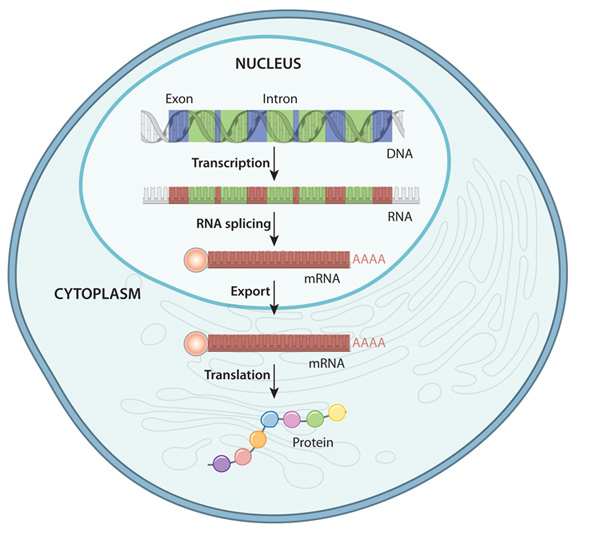
\includegraphics[width=0.8\textwidth]{figures/introduction/gene_expression_process.jpg}
    \caption[Gene expression process]{Overview of gene expression process, from~\cite{cell_essential_nature}}
    \label{fig:gene_expression}
\end{figure}

%%%%%%%%%%%%%%%%%%%%%%%%%%%%%%%%%%%%%%%%%%%%%%%%%%%%%%%%%%%%%%%%%%%%%%%%%%%%%%%%%%%%%%%%%%%%%%%%%%%%%%%%%%%%%%%%%%%%%%%%%%%%%%%%%%%%%%%%%%%%%%%%%%%%%%%%%%%%
%%%%%%%%%%%%%%%%%%%%%%%%%%%%%%%%%%%%%%%%%%%%%%%%%%%%%%%%%%%%%%%%%%%%%%%%%%%%%%%%%%%%%%%%%%%%%%%%%%%%%%%%%%%%%%%%%%%%%%%%%%%%%%%%%%%%%%%%%%%%%%%%%%%%%%%%%%%%
%%%%%%%%%%%%%%%%%%%%%%%%%%%%%%%%%%%%%%%%%%%%%%%%%%%%%%%%%%%%%%%%%%%%%%%%%%%%%%%%%%%%%%%%%%%%%%%%%%%%%%%%%%%%%%%%%%%%%%%%%%%%%%%%%%%%%%%%%%%%%%%%%%%%%%%%%%%%

\subsection{RNA transport mechanisms}
\label{subsec:intro_rna_transport}

When an \ac{mRNA} is ready for export, it is moved out of the nucleus through the nuclear pore complex.
This complex recognizes a mature \ac{mRNA} if a specific set of proteins is bounded to it (poly(a) binding proteins, cap binding proteins, and proteins related to the splicing step).
Once in the cytoplasm, an \ac{mRNA} is not necessarily exploited by a ribosome for translation.
It can also be silenced by translational repressors and stored, transported in a specific region of the cell or degraded.

Until recently, the scientific community thought translation mostly occurred at the endoplasmic reticulum and then proteins were transported where they were needed.
New evidence suggests on the contrary that \ac{mRNA} localization within the cell is not always random and \ac{mRNA}s-proteins colocalization could be an important aspect of cell organization and gene expression regulation \cite{Lecuyer2007}.
However, the involved mechanisms are not well understood yet and the extend of \ac{mRNA}s concerned by a specific localization pattern is still unknown.
Beyond the number of \ac{mRNA} molecules within a cell (the expression level of a gene), researchers manifest now an increasing interest for \ac{mRNA} localization.

\noindent
Some mechanisms used by the cell to transport or locally enrich \ac{mRNA} have already been identified:
\begin{itemize}
	\item Usage of motor proteins to move the \ac{mRNA}s along the cytoskeleton.
	\item Prevention of \ac{mRNA} degradation at a precise location.
	\item Local entrapment to anchor the \ac{mRNA}s.
\end{itemize}

%%%%%%%%%%%%%%%%%%%%%%%%%%%%%%%%%%%%%%%%%%%%%%%%%%%%%%%%%%%%%%%%%%%%%%%%%%%%%%%%%%%%%%%%%%%%%%%%%%%%%%%%%%%%%%%%%%%%%%%%%%%%%%%%%%%%%%%%%%%%%%%%%%%%%%%%%%%%
%%%%%%%%%%%%%%%%%%%%%%%%%%%%%%%%%%%%%%%%%%%%%%%%%%%%%%%%%%%%%%%%%%%%%%%%%%%%%%%%%%%%%%%%%%%%%%%%%%%%%%%%%%%%%%%%%%%%%%%%%%%%%%%%%%%%%%%%%%%%%%%%%%%%%%%%%%%%
%%%%%%%%%%%%%%%%%%%%%%%%%%%%%%%%%%%%%%%%%%%%%%%%%%%%%%%%%%%%%%%%%%%%%%%%%%%%%%%%%%%%%%%%%%%%%%%%%%%%%%%%%%%%%%%%%%%%%%%%%%%%%%%%%%%%%%%%%%%%%%%%%%%%%%%%%%%%

\subsection{Translation}
\label{subsec:intro_translation}

Finally, a cell synthesizes a protein through the translation process.
A ribosome is assembled around a \ac{mRNA} and moves along its nucleotides.
At the same time, \ac{tRNA}s carry amino acids matching the \ac{mRNA} sequence.
According to the genetic code, three successive nucleotides of the \ac{mRNA} (a codon) correspond to an amino acid.
The ribosome sequentially chains the amino acids, which then fold into a protein with a specific 3-dimensional structure.

%%%%%%%%%%%%%%%%%%%%%%%%%%%%%%%%%%%%%%%%%%%%%%%%%%%%%%%%%%%%%%%%%%%%%%%%%%%%%%%%%%%%%%%%%%%%%%%%%%%%%%%%%%%%%%%%%%%%%%%%%%%%%%%%%%%%%%%%%%%%%%%%%%%%%%%%%%%%
%%%%%%%%%%%%%%%%%%%%%%%%%%%%%%%%%%%%%%%%%%%%%%%%%%%%%%%%%%%%%%%%%%%%%%%%%%%%%%%%%%%%%%%%%%%%%%%%%%%%%%%%%%%%%%%%%%%%%%%%%%%%%%%%%%%%%%%%%%%%%%%%%%%%%%%%%%%%
%%%%%%%%%%%%%%%%%%%%%%%%%%%%%%%%%%%%%%%%%%%%%%%%%%%%%%%%%%%%%%%%%%%%%%%%%%%%%%%%%%%%%%%%%%%%%%%%%%%%%%%%%%%%%%%%%%%%%%%%%%%%%%%%%%%%%%%%%%%%%%%%%%%%%%%%%%%%

\subsection{mRNA localization}
\label{subsec:intro_rna_loc}

%%%%%%%%%%%%%%%%%%%%%%%%%%%%%%%%%%%%%%%%%%%%%%%%%%%%%%%%%%%%%%%%%%%%%%%%%%%%%%%%%%%%%%%%%%%%%%%%%%%%%%%%%%%%%%%%%%%%%%%%%%%%%%%%%%%%%%%%%%%%%%%%%%%%%%%%%%%%

% paper racha (introduction)

%how
%- rna metabolism
%- protein metabolism (mature protein or nascent protein)

%why
%- storage of untranslated rna
%- local translation
%- rapid cell division cycle (linked to local translation of cyclin B mRNAs)
%- cell polarization
%- cell motility (actin at the leading edge)
%- axonal growth and synaptic plasticity of neurons
%- assembly of protein complexes
%- avoid proteins in wrong place

%how
%- targeting signal of nascent protein
%- targeting from rna zip-code sequence (with RNA-binding proteins)
%- direct transport on the cytoskeleton by molecular motors
%- anchoring mechanism
%- diffusion, trapping, degradation and local rna stabilization

%claim
%- lack a global view of local translation in the entire cellular space or at the genomic level
%- need a systematic manner

%examples
%- pioneering study in Drosophila
%- human cell lines

%limitations
%- information on RNA localization but did not directly investigate local translation as the encoded proteins were not detected

%%%%%%%%%%%%%%%%%%%%%%%%%%%%%%%%%%%%%%%%%%%%%%%%%%%%%%%%%%%%%%%%%%%%%%%%%%%%%%%%%%%%%%%%%%%%%%%%%%%%%%%%%%%%%%%%%%%%%%%%%%%%%%%%%%%%%%%%%%%%%%%%%%%%%%%%%%%%

% Most mRNAs are distributed randomly throughout the cytoplasm, but some localize to specific
% subcellular areas (Blower, 2013; Bovaird et al., 2018; Eliscovich and Singer, 2017; Jung et al., 2014 for reviews).

% This phenomenon is linked to either RNA metabolism, when untranslated mRNAs are stored in P- bodies or other cellular structures (Hubstenberger et al., 2017),
% or to protein metabolism, when a protein is synthesized locally.

% Local translation has been observed from bacteria and yeast to humans (Blower, 2013; Jung et al., 2014; Eliscovich and Singer, 2017; Bovaird et al., 2018).

% It is commonly involved in the delivery of mature proteins to specific cellular compartments, while allowing local regulation, and this is involved in many processes.
% For instance, it contributes to patterning and cell fate determination during metazoan development, mainly through asymmetric cell division
% (Melton, 1987; Driever and Nu€sslein- Volhard, 1988).
% In Xenopus embryos, local translation of cyclin B mRNAs at the mitotic spindle is also believed to be important for the rapid cell
% division cycles occurring during early embryo- genesis (Groisman et al., 2000).
% In mammals, mRNA localization is involved in cell polarization and motility, mainly through the localization of actin and related mRNAs at the leading edge (Lawrence and Singer, 1986), and it is also involved in axonal
% growth and synaptic plasticity of neurons (Van Driesche and Martin, 2018).

% Importantly, local translation can also be linked to the
% metabolism of the nascent peptide rather than to directly localize the mature protein. For instance, translation of secreted proteins
% at the endoplasmic reticulum (ER) allows nascent pro- teins to translocate through the membrane to reach the ER lumen (Aviram and Schuldiner, 2017).
% Translation of mRNAs at specific sites may also be important for the assembly of protein complexes (Pichon et al., 2016) or
% to avoid the deleterious effects of releasing free proteins at inappropriate places (Mu€ller et al., 2013).

% RNA localization can be accomplished through several mech- anisms. In the case of secreted proteins, the nascent peptide serves as a
% targeting signal, via the signal recognition particle (SRP) and its receptor on the ER (Aviram and Schuldiner, 2017).

% In most other cases, targeting is an RNA-driven process (Blower, 2013; Jung et al., 2014; Eliscovich and Singer, 2017; Bovaird et al., 2018 for reviews).
% Localized mRNAs often contain a zip-code sequence, frequently located within their 30-UTR, which is necessary and sufficient to transport them to their destination.
% The zip code is recognized by one or several RNA-binding proteins (RBPs), and it drives the formation of a transport complex sometimes called locasome.
% This complex can be transported by centrosomes, endosomal vesicles, or other cellular structures (Blower, 2013; Jung et al., 2014; Eliscovich and Singer, 2017; Bovaird et al., 2018).

% However, direct transport on the cytoskeleton by molecular motors is a frequent mechanism (Blower, 2013; Bovaird et al., 2018; Eliscovich and Singer, 2017; Jung et al., 2014).

% Once at destination, an anchoring mechanism may limit diffusion away from the target site.

% Alternatives to these transport mechanisms include diffusion and trap- ping at specific locations and degradation coupled to local RNA stabilization.

% Localized mRNAs are often subjected to a spatial control of translation (Besse and Ephrussi, 2008).
% In the case of Ash1 mRNA in yeast and b-actin mRNA in neurons, translation is repressed during transport and
% is activated at their final location by phosphorylation-dependent mechanisms (Hu€ttelmaier et al., 2005; Paquin et al., 2007).
% This spatial regulation of translation provides an additional layer of control ensuring that mRNAs are translated only at the desired location.

% The first locally translated mRNAs were found by chance or using a candidate approach.
% Purification of cellular structures and localized RBPs have significantly increased the number of known localized mRNAs
% (Blower, 2013; Jung et al., 2014; Eliscovich and Singer, 2017; Bovaird et al., 2018).

% However, only specific compartments or RBPs were examined, and we currently lack a global view of local translation in the entire cellular space or at the genomic level.
% Few reports described attempts to characterize mRNA localization in a systematic manner.

% A pioneering study in Drosophila used whole-mount fluorescent in situ hybrid- ization (FISH) to analyze the localization of more than 2,000 mRNAs (Lecuyer et al., 2007).
% As many as 71\% of them had a non-random distribution, and a range of new localization patterns were observed.
% More recent reports confirmed that RNA localization is widespread during Drosophila development (Jam- bor et al., 2015; Wilk et al., 2016).

% However, it is not known whether this is also true in other organisms, particularly in humans. Few recent studies addressed this question in cell lines
% using the more sensitive single-molecule FISH technique (smFISH). Several thousands of mRNAs were analyzed, which
% showed a correlation of intracellular mRNA distribution with gene annotation (Battich et al., 2013; Chen et al., 2015; Eng et al., 2019; Xia et al., 2019).
% Specifically, these studies identified three groups of localized mRNAs, in the perinuclear area, the mitochondria, and the cell periphery,
% the latter being possibly linked to actin metabolism (Chen et al., 2015).

% These studies provided information on RNA localization but did not directly investigate local translation as the encoded proteins were not detected.
% Thus, we still lack a good understanding of the various functions played by local translation at the cellular level.

% In this study, we developed a smFISH screen to specifically address this issue. Using a set of 523 GFP-tagged cell lines spanning
% a variety of cellular functions and an approach that allows simultaneous visualization of mRNA and proteins,
% we found that local translation occurs at various unanticipated locations. In particular, we discovered specialized
% translation factories, where specific mRNAs are translated. These factories are remarkable in that they provide
% a unique mean to regulate the metabolism of nascent proteins and also create a fine granular compartmentalization of translation.

%%%%%%%%%%%%%%%%%%%%%%%%%%%%%%%%%%%%%%%%%%%%%%%%%%%%%%%%%%%%%%%%%%%%%%%%%%%%%%%%%%%%%%%%%%%%%%%%%%%%%%%%%%%%%%%%%%%%%%%%%%%%%%%%%%%%%%%%%%%%%%%%%%%%%%%%%%%%

% paper racha (dual protein-rna localization screens)

% In order to simultaneously visualize mRNAs with their encoded proteins, we based our screen on a library of HeLa cell lines,
% each containing a bacterial artificial chromosome (BAC) stably integrated in their genome (Poser et al., 2008).
% Each BAC con- tains a GFP-tagged gene harboring all its regulatory sequences (promoter, enhancers, introns, and 50 and 30 UTRs; Figure 1A).
% The resulting mRNAs are, thus, identical to the endogenous mol- ecules in terms of sequence and isoform diversity, except for the added tag.
% Previous studies showed that such tagged genes are expressed at near endogenous levels and with the proper spatio- temporal pattern (Poser et al., 2008).
% Since the tagged mRNAs contain all the regulatory sequences, we hypothesized that they would localize like the endogenous ones,
% provided that the tag does not interfere with localization. Using BACs offers two advantages. First, a single smFISH probe set
% against the GFP sequence is sufficient to detect all the studied mRNAs. Sec- ond, using mild hybridization conditions,
% GFP fluorescence can be detected together with the smFISH signal (Fusco et al., 2003), and thus, both the mRNA and the encoded protein can be detected in the same cell.

% paper racha (DYNC1H1 motor protein)

% Molecular motors transport cargos to different cellular destina- tions and accumulate themselves at various cellular locations.
% The third pattern, referred to as ‘‘foci,’’ was observed for the dynein heavy-chain mRNA (DYNC1H1).
% This mRNA localized throughout the cytoplasm but aggregated in some bright structures containing several mRNA molecules (Figure 1C), as reported recently (Pichon et al., 2016).

% paper racha (systematic screeening)

% Overall, accumulation of mRNAs in foci was the most frequent pattern (19 out of the total of 32 localized mRNAs; Tables 1 and S2).
% To determine whether any of these foci were P-bodies, we imaged mRNAs together with a P-body marker. Indeed, foci of
% 15 mRNAs co-localized with P-bodies (Figure S5), while the remaining four were distinct structures (BUB1, DYNC1H1, CTNNB1/b-catenin, and ASPM mRNA; Figure S6A).

% paper racha (locally translated mRNAs)

% Having analyzed the localization patterns by a quantitative and unbiased approach, we then examined the co-localization of
% the mRNAs with their encoded protein. Although accumulation of mRNAs in foci was the most frequent pattern (19/32; see Table 1),
% only two mRNAs displayed a faint but detectable GFP signal in their foci: CRKL and CTNNB1/b-catenin (see Figures 2B and S4 for
% CRKL and Figure S11A for CTNNB1/b-catenin). For the other localization patterns, 9 mRNAs co-localized with their pro- tein
% (2\% of the screened mRNAs; Table 1): AKAP1, AKAP9, AP1S2, ASPM, ATP6A2, FLNA, HMMR, NUMA1, and HSP90B1 (Figure 2).
% In some cases, the mRNA/protein co-local- ization was expected. For instance, both HSP90B1 and ATP6A2 contain a signal peptide
% leading to translation on the ER, and HSP90B1 is a resident ER protein while ATP6A2 localizes in endo-lysosomes close to this
% compartment (Figure 2B). Similarly, AKAP1 encodes an RNA-binding protein localizing to the surface of mitochondria, and
% this transcript thus belongs to the known class of mitochondrion-localized mRNAs (Sylvestre et al., 2003). The other proteins
% localized to cellular structures that were not previously known to use local translation as a tar- geting mechanism.
% This included the clathrin adaptor AP1S2 mRNA that localized on endosomes and the AKAP9 mRNA that accumulated at the Golgi.
% Below, we explore these cases in more detail together with mRNAs localizing around centro- somes (ASPM, NUMA1, and HMMR),
% at the nuclear envelope (ASPM and SPEN), or in cytoplasmic foci that were not P-bodies (ASPM, BUB1, DYNC1H1, and CTNNB1/b-catenin).

% racha paper (nuclear envelope rna)

% The Localization of ASPM and SPEN mRNAs at the Nuclear Envelope Is Translation-Dependent
% ASPM-GFP mRNAs accumulated at the nuclear envelope during interphase (Figure 2C; quantification in Figure 3E). In addition,
% SPEN-GFP mRNAs, which encode a nuclear protein, were also enriched around the nuclear envelope (Figures 2B and 3E).
% Labeling of the nuclear pores using either a CRM1-GFP fusion or an antibody against NUP133 (Figures S9A and S9B) showed
% that ASPM and SPEN mRNAs localized close to nuclear pores, rather than between them. This localization could result from
% two mechanisms. First, mRNAs could transiently localize at the pores on their way out of the nucleus. Second, they could
% localize at the cytoplasmic side of the pore to facilitate re-entry of newly translated proteins. To distinguish between
% these pos- sibilities, we inhibited either transcription with actinomycin D, or translation with puromycin. After 1 h of
% actinomycin D treatment, SPEN and ASPM mRNAs still localized at the nuclear envelope (left panels in Figures 4A, S9C, and
% 4B for quantifications). On the contrary, both mRNAs became dispersed after 1-h exposure to puromycin (Figures 4A, 4B, S9C,
% and S10A for quantifica- tions). We then used cycloheximide, which inhibits translation by freezing the ribosomes on the mRNAs,
% in contrast to puromy- cin that induces premature termination and releases the nascent peptide. Cycloheximide had no effects
% on the localization of ASPM mRNAs (Figures 4A left panels and 4B), indicating that their localization did not require protein
% synthesis per se, but more likely the presence of nascent proteins on polysomes. Therefore, ASPM and SPEN mRNAs at the nuclear
% envelope are not in transit to the cytoplasm but localize on the nuclear en- velope by a translation-dependent mechanism requiring the nascent protein.

% ASPM mRNAs Are Translated at the Nuclear Envelope
% We and others recently demonstrated that the SunTag can be used to visualize translation of single mRNPs in live cells
% (Pichon et al., 2016; Wu et al., 2016; Yan et al., 2016; reviewed in Pichon et al., 2018). The SunTag is a repeated
% epitope and in cells ex- pressing an scFV-GFP monochain antibody directed against this epitope, the antibody binds
% the repeated tag as soon as it emerges from the ribosome, allowing the visualization of single molecules of nascent proteins
% (e.g., monosome and polysomes). To confirm that ASPM mRNAs were translated at the nuclear en- velope, we tagged the
% endogenous gene using CRISPR genome editing. Homologous recombination allowed to obtain heterozy- gous clones where
% 32 SunTag repeats were fused at the N termi- nus of ASPM proteins (Figure S9D). The endogenous ASPM tran- scripts
% were then labeled by smiFISH, revealing both tagged and untagged mRNAs. This showed that bright spots of scFv-GFP
% co-localized with single ASPM mRNAs (Figure 4C; white arrows). These spots disappeared after a 20 min puromycin
% treatment, confirming that they were polysomes (Figure S9E). We then per- formed time-lapse analyses of live cells,
% recording one image stack every 40 s for 50 min (see Video S1 and still images in Fig- ure 4D). Remarkably,
% some polysomes localized at the nuclear envelope. While cytoplasmic polysomes moved too rapidly to be tracked, the ones at the envelope remained immobile for
% extended periods of times (29 min on average). Thus, a fraction of ASPM mRNAs was stably anchored and translated at the nu- clear envelope.

% racha paper (use of puromycin)

% Translation Inhibition with Puromycin Frequently Prevents mRNA Localization
% Since the localization of ASPM mRNA at the envelope is transla- tion dependent, we tested whether this was also the case for its
% localization at centrosomes. Puromycin abolished its localiza- tion, while actinomycin D and cycloheximide had little effect
% (Fig- ure 4A, right panels; Figure 4B for quantification). The effect of puromycin was then tested on the other localized mRNAs.
% After 1 h of treatment, KIF1C and MYH3 mRNAs still localized to cyto- plasmic protrusions (Figures 5A and 5B for quantifications).
% In contrast, HSP90B1, HMMR, AP1S2, AKAP1, KIF4A, and AKAP9 mRNAs all became delocalized and lost co-localization with their
% ncoded protein when translation was inhibited (Fig- ures 5C–5E and S10A–S10D). The data demonstrated are consistent with the
% hypothesis that translation is required for the localization of these mRNAs.

% racha paper (translation factories)

% Non-P-Body mRNA Foci Correspond to Specialized Translation Factories
% Four mRNAs accumulated in foci that were distinct from P- bodies (BUB1, DYNC1H1, CTNNB1/b-catenin, and ASPM; Fig- ure S6A).
% The dynein heavy-chain DYNC1H1 and the ASPM pro- tein were described above. BUB1 is a checkpoint kinase that
% verifies the attachment of microtubules to kinetochores at the onset of mitosis (Saurin, 2018), and b-catenin is the
% key tran- scription factor of the Wnt signaling pathway (Grainger and Wil- lert, 2018). SmiFISH confirmed that the four
% endogenous mRNAs accumulated in foci (Figures S2A, S8C, S10E, and see below S11F). Moreover, dual-color smiFISH showed
% that these foci did not co-localize together, indicating that they were distinct structures (Figure 6A).
% We then inhibited translation with puro- mycin, using an mRNA accumulating in P-bodies as control (AURKA).
% After 1 h of treatment, the non-P-body foci virtually dis- appeared (Figures 6B and 6C), while the accumulation
% of AURKA mRNA in P-bodies actually increased. Thus, translation inhibition specifically disrupted the mRNA foci
% that were not P-bodies. We previously used the SunTag to show that DYNC1H1 is translated in the mRNA foci (Pichon et al., 2016).
% Using the CRISPR SunTag clone described above, we found that ASPM mRNAs were simi- larly translated in the mRNA foci
% (Figure 4C, orange arrow; 70\% of the foci have a SunTag signal). A 32xSunTag repeat was then introduced at the N terminus of the BUB1
% protein using CRISPR gene editing. BUB1 mRNAs were detected by smiFISH and were found to be frequently translated in the foci
% (Figures 6D and 6E; 70\% of the foci contained a SunTag signal), in contrast to mRNAs located outside foci for which the SunTag signal was
% rarely detected (1\% of the time). Taken together, these data demonstrated that ASPM, BUB1, and DYNC1H1 are translated
% in mRNA foci, which thus correspond to specialized translation factories.

% racha paper (CTNNB1)

% We then analyzed in more details CTNNB1/b-catenin. This pro- tein has two roles: it bridges E-cadherin to the actin cytoskeleton
% at adherens junctions, and it acts as the main transcription factor of the Wnt pathway (for review, see Grainger and Willert, 2018; MacDonald et al., 2009).
% The Wnt signaling pathway is essential during development, is often a key actor during tumorigenesis, and involves a fast
% activation of b-catenin expression by Wnt. The b-catenin protein localized at adherens junction is stable whereas the one
% synthesized in the cytoplasm is rapidly degraded (reviewed in Stamos and Weis, 2013). However, the cytoplasmic protein is
% stabilized in presence of a Wnt signal and can then accumulate in the nucleus to activate transcription of target genes.
% In the b-catenin BAC cells, the GFP-tagged pro- tein was weakly expressed. It accumulated at sites of cell-cell contacts
% as expected and also showed a weak staining in the brightest RNA foci (Figure S11A). Because the maturation of the GFP
% chromophore is slow and therefore inadequate to map translation sites, we combined smFISH with immunofluo- rescence,
% using an antibody binding the N terminus of b-catenin. The mRNA foci contained high levels of b-catenin N termini (Fig- ure S11B).
% Since these foci were also dissolved when translation was inhibited (see Figures 6B and 6C), these data indicated that b-catenin was translated in the mRNA foci.
% Interestingly, there was a small fraction of the BAC cells where b-catenin mRNAs did not form foci and instead were dispersed as single molecules in the cytoplasm.
% Furthermore, these cells ex- pressed high levels of nuclear b-catenin-GFP, suggesting that the Wnt pathway had been activated and
% was responsible for the disappearance of the foci (Figure S11C). To test this hypothe- sis, we activated the Wnt pathway by
% incubating the BAC cell line with the WNT3A protein. Indeed, the mRNA foci disappeared after 30 min, concomitant with a
% higher expression of b-catenin-GFP and its accumulation in the nucleus (Figures 7A and 7E for quan- tifications).
% This observation established a link between the pres- ence of mRNA foci and the degradation of the b-catenin protein.
% One hypothesis to explain these results would be that b-catenin
% degradation takes place co-translationally in the foci. Degradation of b-catenin requires Axin, APC, and the kinases
% CK1a and GSK3, which altogether form the ‘‘destruction complex’’ (Stamos and Weis, 2013).
% In absence of Wnt, this complex binds b-catenin and targets it for degradation. In presence of Wnt, its components become recruited to the
% plasma membrane, and they can no longer interact with b-catenin (Grainger and Willert, 2018; Stamos and Weis, 2013; MacDonald et al., 2009).
% Axin is an essential player of the destruction complex, and it acts as a scaffolding pro- tein
% (Grainger and Willert, 2018; Stamos and Weis, 2013; Mac- Donald et al., 2009).
% It binds b-catenin as well as APC, CK1a, and GSK3, and its role is to bring b-catenin in proximity to the ki- nases CK1a and GSK3 (3–5).
% b-catenin is first phosphorylated on residue S45 by CK1a, leading to its recognition by GSK3, which phosphorylates
% it on residues T41, S37, and S33. Phosphorylated b-catenin is then recognized by the E3 ubiquitin ligase b-TrCP,
% which targets it for proteasomal degradation. APC is a very large protein that is essential for b-catenin degradation
% but whose exact molecular function is unclear. It occurs as a dimer and each mono- mer has more than 30 tandemly
% repeated binding sites for b-catenin.
% Labeling with anti-APC or anti-Axin1 antibodies revealed that the b-catenin mRNA foci contained high levels of APC
% and were also enriched for Axin1 (Figure 7B). Moreover, Axin1 could be detected in polysomal fractions in a
% translation-dependent manner (Figure S11D), suggesting that it binds b-catenin co- translationally.
% We then immuno-localized phosphorylated b-catenin (on residues S33 and S37), to test its presence in the mRNA foci.
% In this case, we used N-terminal labeling of b-catenin as a proxy for the mRNA foci because the anti-phospho anti- bodies
% were not compatible with smFISH (Figure 7C). Indeed, phospho-b-catenin accumulated in the mRNA foci.
% In addition, we could also detect cross-linked chains of ubiquitin itself (Fig- ure 7C).
% Altogether these data indicated that the mRNA foci were sites of both b-catenin synthesis and degradation, i.e., sites of co-translational protein degradation.
% Foci formation was further regulated by Wnt signaling, thereby allowing a fast post-translational response.
% Interestingly, Axin can oligomerize and APC can cross-link these oligomers to make large aggregates (Grainger and Willert, 2018; Stamos and Weis, 2013; MacDonald et al., 2009),
% suggesting that these factors could be involved in foci formation. Indeed, when APC was knocked down with siRNA,
% we observed a 50-fold increase of b-catenin levels and, remarkably, a disap- pearance of the mRNA foci (Figures 7D and 7F).
% Likewise, mRNA foci were disrupted upon Axin1 knockdown. In contrast, when we increased Axin1 levels by inhibiting
% Tankyrase with the small molecule LG-007 (Huang et al., 2009), the endogenous b-catenin mRNA formed more foci in HEK293 cells:
% foci were visible in 16\% of the cases in untreated cells, and this increased to 32\% after LG-007 treatment for 2 h (Figures S11F and S11G).
% Finally, we also tested a pharmacological inhibition of GSK3. Indeed, APC and Axin1 are themselves phosphorylated by GSK3, and this
% promotes complex formation and their interac- tion with b-catenin (Ha et al., 2004; Wu and Pan, 2010). Remark- ably, GSK3 inhibition
% for 1 h nearly completely dissolved b-cate- nin mRNA foci. These data suggest that foci formation relies on the co-translational
% recognition of b-catenin by APC and Axin1, and the multimerization of these factors.

%%%%%%%%%%%%%%%%%%%%%%%%%%%%%%%%%%%%%%%%%%%%%%%%%%%%%%%%%%%%%%%%%%%%%%%%%%%%%%%%%%%%%%%%%%%%%%%%%%%%%%%%%%%%%%%%%%%%%%%%%%%%%%%%%%%%%%%%%%%%%%%%%%%%%%%%%%%%

% other

% https://www.sciencedirect.com/science/article/pii/S2589004221012670

%%%%%%%%%%%%%%%%%%%%%%%%%%%%%%%%%%%%%%%%%%%%%%%%%%%%%%%%%%%%%%%%%%%%%%%%%%%%%%%%%%%%%%%%%%%%%%%%%%%%%%%%%%%%%%%%%%%%%%%%%%%%%%%%%%%%%%%%%%%%%%%%%%%%%%%%%%%%

% paper xavier (introduction)

% Localization of mRNA to specific subcellular compart- ments is an important mechanism for the spatio-temporal regulation of
% gene expression in diverse cell types and or- ganisms (Chin and Lécuyer 2017; Eliscovich and Singer 2017).
% Subcellular mRNA localization allows localized pro- tein synthesis and this is important for many biological
% functions such as cell fate determination (Berleth et al. 1988), cell polarization (Condeelis and Singer 2005),
% cell division (Chouaib et al. 2020; Ryder et al. 2020), cell migration (Katz et al. 2012; Wang et al. 2017; Moissoglu et al. 2020),
% embryonic patterning (Forrest and Gavis 2003), and synaptic plasticity (Martin and Zukin 2006; Lin and Holt 2007).

% One of the best characterized examples is the yeast Ash1 mRNA that localizes specifically in the bud of the daughter
% cells and encodes a transcriptional re- pressor protein involved in suppressing mating-type switching (Paquin and Chartrand 2008).

% Studies of this and other models revealed that the subcellular localization of mRNA relies on three main mechanisms, acting
% separately or in combination: random diffusion combined with local entrapment, general transcript degradation
% coupled to localized protection and directed transport along the cytoskeleton (Medioni et al. 2012; Cody et al. 2013; Bovaird et al. 2018).

% Active, motor-driven transport of mRNAs along the cyto- skeleton is thus far the most common localization mecha- nism.
% It generally involves cis-acting elements, also called zipcodes, contained in the 3′UTR sequence of the transcript.
% This is exemplified by the case of the β-actin mRNA in vertebrates, which accumulates at the leading edge of migrating
% cells and was among the first localized mRNAs discovered (Singer 1993). This mRNA contains a zipcode sequence recognized
% by the RNA Binding Protein ZBP1, allowing the transport of β-actin mRNAs in a motor-driven manner along the
% cytoskeleton (Kislauskis et al. 1993; Oleynikov and Singer 2003; Condeelis and Singer 2005; Liao et al. 2015).

% Interestingly, transport of β-actin mRNA by ZBP1 involves both microtubules (MTs) and actin filaments
% (Fusco et al. 2003; Oleynikov and Singer 2003), as well as several motors that display some cell type and com- partment specificity.
% Indeed, MYO5A and KIF5A interact with ZBP1 to transport β-actin mRNAs in dendrites and ax- ons (Ma et al. 2011; Nalavadi et al. 2012),
% while Myosin IIB (MYH10) and KIF11, which directly binds ZBP1, regulate the transport of β-actin mRNAs in fibroblasts
% and during cell migration (Latham et al. 2001; Song et al. 2015).

% In vertebrate systems, the motors involved in RNA trans- port have been investigated mostly in neuronal cells. Kine- sin-1 (KIF5) was
% shown to associate with neuronal RNP granules and to be involved in their trafficking (Kanai et al. 2004). Kinesin-1 was also
% implicated in transport of myelin basic protein (MBP) mRNA in oligodendrocytes (Carson et al. 1997) as well as in shank1 mRNA
% transport in rat neurons (Falley et al. 2009). Kinesin-2 (KIF3A/B/ KAP3) can transport RNAs in vitro (Baumann et al. 2020),
% but its in vivo relevance is still unclear. The involvement of additional motors, and the means through which they connect
% to potential RNA cargoes are still largely unex- plored, especially in the case of nonneuronal cell types (Gagnon and Mowry 2011; Xing and Bassell 2013).

% Localized RNAs are prevalent in nonneuronal, mesenchy- mal cells. Apart from β-actin, numerous other RNAs are local- ized at
% protrusions of mesenchymal cells and their local translation is important for cell migration (Mili et al. 2008; Mardakheh et al. 2015; Costa et al. 2020; Moissoglu et al. 2020).

% Localization of these RNAs is carried out through at least two distinct pathways. Specifically, a subset of about a hundred RNAs,
% which include transcripts encoding signal- ing and cytoskeleton regulators (such as the Rab GTPase RAB13, the RhoA exchange factor NET1,
% the collagen re- ceptor DDR2, the motor related proteins TRAK2, DYNLL2, and others), require the APC tumor suppressor protein for
% lo- calization and have been referred to as APC-dependent (Wang et al. 2017). Other protrusion-enriched RNAs, exem- plified by
% RNAs encoding ribosomal proteins, do not require APC and exhibit distinct regulation (Wang et al. 2017).

% Similar to what has been described for other localized RNAs, sequences within the 3′UTR of APC-dependent RNAs are necessary
% and sufficient for targeting to the cell periphery (Mili et al. 2008). Specifically, interfering with or deleting particular
% GA-rich regions is sufficient to disrupt peripheral localization and perturb cell movement in vari- ous systems
% (Chrisafis et al. 2020; Costa et al. 2020; Moisso- glu et al. 2020).

% Furthermore, localization to the periphery requires
% the microtubule cytoskeleton and in particular a subset of stable, detyrosinated microtubules (Wang et al. 2017; Moissoglu et al. 2019).

% Indeed, at least some APC- dependent RNAs exhibit a colocalization with the plus ends of detyrosinated microtubules (Mili et al. 2008).
% The peripheral complexes also contain APC, a protein that has the ability to directly bind microtubules via its carboxyl terminus
% (Munemitsu et al. 1994; Zumbrunn et al. 2001; Jimbo et al. 2002; Barth et al. 2008; Bahmanyar et al. 2009), hence suggesting that
% APC might mediate the inter- action of localized mRNAs with microtubules (Mili et al. 2008; Preitner et al. 2014).

% An additional feature integrated with the localization of APC-dependent RNAs is their existence in distinct physical states.
% In particular, RNAs in internal or peripheral, actively extending cytoplasmic regions exist as single molecules that are undergoing
% translation. However, at some periph- eral areas, single RNAs coalesce in multimeric heteroge- neous clusters that are composed of
% multiple distinct RNA species. Interestingly, these clusters preferentially form at retracting protrusions and contain
% translationally si- lent mRNAs (Moissoglu et al. 2019).

% These data indicate the existence of a dynamic regulatory mechanism during
% cell migration, which coordinates local mRNA translation with protrusion formation and retraction. However, the exact mechanisms
% and molecular players involved in transport to the periphery and cluster formation for this group of RNAs are still unclear.

% In this study, we focused on the kinesin KIF1C, which we recently showed to accumulate and colocalize with its own mRNA in cytoplasmic
% protrusions (Chouaib et al. 2020). We show here that KIF1C associates with additional protrusion-localized RNAs belonging to
% the APC-dependent group. We describe a specific mRNA transport mechanism by which the KIF1C kinesin motor binds APC-dependent mRNAs,
% including its own, actively transports them to cell protrusions in a 3′UTR dependent manner and additionally participates
% in promoting and/or maintaining their peripheral clusters.

%%%%%%%%%%%%%%%%%%%%%%%%%%%%%%%%%%%%%%%%%%%%%%%%%%%%%%%%%%%%%%%%%%%%%%%%%%%%%%%%%%%%%%%%%%%%%%%%%%%%%%%%%%%%%%%%%%%%%%%%%%%%%%%%%%%%%%%%%%%%%%%%%%%%%%%%%%%%

%~\cite{Medioni_2012}

% Transporting mRNAs rather than proteins presents several significant advantages for a cell.
% First, transport costs are reduced, as several protein molecules can be translated from a single RNA molecule.
% Second, transporting mRNAs can prevent proteins from acting ectopically before they reach the appropriate site,
% which is particularly important in the case of maternal determinants, as spatially inappropriate expression disrupts embryonic patterning.
% Third, localized translation can facilitate incorporation of proteins into macromolecular complexes by generating high local
% protein concentrations and allowing co-translation of different subunits (Mingle et al., 2005).
% Fourth, nascent proteins may have properties distinct from pre-existing copies, by virtue of post-translational
% modifications or through chaperone-aided folding pathways (Lin and Holt, 2007).
% Lastly, a major advantage of mRNA targeting is that it allows fine-tuning of gene expression in both space and time.
% Examples of this include targeting of different splice variants to distinct cellular compartments (Baj et al., 2011)
% and activation of localized mRNA translation specifically at their destination, in response to signals
% such as guidance cues, neurotransmitter release or fertilization (Besse and Ephrussi, 2008).

%%%%%%%%%%%%%%%%%%%%%%%%%%%%%%%%%%%%%%%%%%%%%%%%%%%%%%%%%%%%%%%%%%%%%%%%%%%%%%%%%%%%%%%%%%%%%%%%%%%%%%%%%%%%%%%%%%%%%%%%%%%%%%%%%%%%%%%%%%%%%%%%%%%%%%%%%%%%

% thesis adham

%2. mRNA localization in cell lines: generalities
%The two mRNA localization screens provided insights into general mRNA localization features in cell lines:

%First, even in the case of mRNAs that produce a strong pattern (DYNC1H1 mRNAs localizing in foci for example), a non-negligible fraction of mRNA molecules always seems to have random distribution. This is not the case in other systems such as developing embryos or oocytes in which most molecules of a localized transcript actually display the pattern. The reasons behind this difference are unclear; but (i) they could be a general aspect of mRNA localization in cell lines, in which they are much less stereotyped than embryos, especially cancer ones like HeLa; (ii) they could arise due to the relatively smaller size of HeLa cells (although similar observations are made in neurons which argues against this); (iii) localizing only a fraction of mRNA molecules is sufficient to carry out the intended biological function (discussed in detail below), in which there is no need to localize all transcripts for the cell to function properly.

%mRNA localization occurs in a wide range of subcellular locations in cell lines. These include cellular protrusions, the Golgi apparatus, endosomes, the nuclear envelope, cell edges, centrosomes, and even the cytosolic space itself (as in the case of mRNA foci and polarized distributions). This demonstrates the variety of mRNA trafficking and the diverse functions of mRNA localization.

%Most localized mRNAs display ìsimpleî localization patterns in which they belong to one of the described localization classes (intranuclear, nuclear envelope, cell edge, cell extension, polarized, foci, centrosomes). However, some transcripts show ìcomplexî patterns in which they localize to multiple compartments either simultaneously or at different times. An example of this is HMMR mRNA that localizes to both centrosomes and P-bodies during interphase. This difference is probably related to the function of each transcript but it implies that mRNA localization can be complex and can involve multiple sub-cellular compartments at once (see ASPM below for a detailed example).

%mRNA localization often exhibits cellular heterogeneity. Indeed, not all cells exhibit the pattern, and the strength of the pattern could vary between cells that display it. The is probably related to: (i) cells having different physiological states and thus different gene expression needs; (ii) cells being in different stages of the cell cycle; (iii) variations in mRNA
%expression levels; (iv) variation in motors protein availability, RBP expression, cytoskeletal arrangements; or (v) a stochastic process yet unidentified.

%3. A variety of local translation flavors
%In many cases, mRNAs co-localized with the protein they encode suggesting local translation. This was observed in a variety of regions such as cell extensions, cell edges, centrosomes, endosomes, and the Golgi network. Local translation could function in:

%Protein targeting: ASPM mRNA for instance was the first case of local translation at the nuclear pore during interphase and this could facilitate nucleoplasmic targeting of the mature ASPM protein.

%Preventing aberrant dispersal of proteins that could have harmful effects. For example, NUMA1 mRNA and protein are only localized on centrosomes during mitosis. Targeting NUMA1 protein to centrosomes during interphase could have deleterious effects.

%Enhancing translation efficiencies: this applies to mRNAs that are localized and translated in cytoplasmic foci referred to as translation factories. These structures could host an environment more suitable for translation (a more favorable concentration of translation factors for instance). In fact, DYNC1H1 mRNAs are translated as both single molecules and mRNA foci. However, mRNAs in the foci are more often found engaged in translation than ones that exist as single molecules. Here, it is tempting to speculate that translation factories harbor specialized ribosomes or components of the translation machinery that are dedicated for localized cases of protein synthesis.

%Nascent peptide metabolism: synthesizing components of a protein complex locally can enhance the efficiency of complex assembly for example. Another possibility is co- translational assembly at certain organelles. For instance, translating mRNAs encoding centrosomal proteins such as PCNT, CEP350, NIN, and HMMR could help to incorporate the mature protein into centrosomes during the expansion of the pericentriolar material that occurs during the late G2 phase of the cell cycle. Finally, local translation could allow certain

%%%%%%%%%%%%%%%%%%%%%%%%%%%%%%%%%%%%%%%%%%%%%%%%%%%%%%%%%%%%%%%%%%%%%%%%%%%%%%%%%%%%%%%%%%%%%%%%%%%%%%%%%%%%%%%%%%%%%%%%%%%%%%%%%%%%%%%%%%%%%%%%%%%%%%%%%%%%
%%%%%%%%%%%%%%%%%%%%%%%%%%%%%%%%%%%%%%%%%%%%%%%%%%%%%%%%%%%%%%%%%%%%%%%%%%%%%%%%%%%%%%%%%%%%%%%%%%%%%%%%%%%%%%%%%%%%%%%%%%%%%%%%%%%%%%%%%%%%%%%%%%%%%%%%%%%%
%%%%%%%%%%%%%%%%%%%%%%%%%%%%%%%%%%%%%%%%%%%%%%%%%%%%%%%%%%%%%%%%%%%%%%%%%%%%%%%%%%%%%%%%%%%%%%%%%%%%%%%%%%%%%%%%%%%%%%%%%%%%%%%%%%%%%%%%%%%%%%%%%%%%%%%%%%%%

\section{Imaging cells and RNAs}
\label{sec:fish}

\begin{center}
	\textit{(To be completed)}
\end{center}

% paper racha (dual protein-rna localization screens)

% In order to simultaneously visualize mRNAs with their encoded proteins, we based our screen on a library of HeLa cell lines,
% each containing a bacterial artificial chromosome (BAC) stably integrated in their genome (Poser et al., 2008).
% Each BAC con- tains a GFP-tagged gene harboring all its regulatory sequences (promoter, enhancers, introns, and 50 and 30 UTRs; Figure 1A).
% The resulting mRNAs are, thus, identical to the endogenous mol- ecules in terms of sequence and isoform diversity, except for the added tag.
% Previous studies showed that such tagged genes are expressed at near endogenous levels and with the proper spatio- temporal pattern (Poser et al., 2008).
% Since the tagged mRNAs contain all the regulatory sequences, we hypothesized that they would localize like the endogenous ones,
% provided that the tag does not interfere with localization. Using BACs offers two advantages. First, a single smFISH probe set
% against the GFP sequence is sufficient to detect all the studied mRNAs. Sec- ond, using mild hybridization conditions,
% GFP fluorescence can be detected together with the smFISH signal (Fusco et al., 2003), and thus, both the mRNA and the encoded protein can be detected in the same cell.

%%%%%%%%%%%%%%%%%%%%%%%%%%%%%%%%%%%%%%%%%%%%%%%%%%%%%%%%%%%%%%%%%%%%%%%%%%%%%%%%%%%%%%%%%%%%%%%%%%%%%%%%%%%%%%%%%%%%%%%%%%%%%%%%%%%%%%%%%%%%%%%%%%%%%%%%%%%%
%%%%%%%%%%%%%%%%%%%%%%%%%%%%%%%%%%%%%%%%%%%%%%%%%%%%%%%%%%%%%%%%%%%%%%%%%%%%%%%%%%%%%%%%%%%%%%%%%%%%%%%%%%%%%%%%%%%%%%%%%%%%%%%%%%%%%%%%%%%%%%%%%%%%%%%%%%%%
%%%%%%%%%%%%%%%%%%%%%%%%%%%%%%%%%%%%%%%%%%%%%%%%%%%%%%%%%%%%%%%%%%%%%%%%%%%%%%%%%%%%%%%%%%%%%%%%%%%%%%%%%%%%%%%%%%%%%%%%%%%%%%%%%%%%%%%%%%%%%%%%%%%%%%%%%%%%

\subsection{Fluorescent proteins}
\label{subsec:intro_fluorescence}

\subsection{A zoo of FISH}
\label{subsec:intro_fish}

% thesis adham: "the invention of single molecule FISH (Femino et al., 1998)"

%%%%%%%%%%%%%%%%%%%%%%%%%%%%%%%%%%%%%%%%%%%%%%%%%%%%%%%%%%%%%%%%%%%%%%%%%%%%%%%%%%%%%%%%%%%%%%%%%%%%%%%%%%%%%%%%%%%%%%%%%%%%%%%%%%%%%%%%%%%%%%%%%%%%%%%%%%%%
%%%%%%%%%%%%%%%%%%%%%%%%%%%%%%%%%%%%%%%%%%%%%%%%%%%%%%%%%%%%%%%%%%%%%%%%%%%%%%%%%%%%%%%%%%%%%%%%%%%%%%%%%%%%%%%%%%%%%%%%%%%%%%%%%%%%%%%%%%%%%%%%%%%%%%%%%%%%
%%%%%%%%%%%%%%%%%%%%%%%%%%%%%%%%%%%%%%%%%%%%%%%%%%%%%%%%%%%%%%%%%%%%%%%%%%%%%%%%%%%%%%%%%%%%%%%%%%%%%%%%%%%%%%%%%%%%%%%%%%%%%%%%%%%%%%%%%%%%%%%%%%%%%%%%%%%%

\section{Measuring images: from pixels to numbers}
\label{sec:computation_biology}

\begin{center}
	\textit{(To be completed)}
\end{center}

% learning principles + generic modules of deep learning + flexible architecture
% advantage/limitations over traditionnal methods -> need to train (heterogeneity of dataset // self or weaekly supervised methods, simulations)
% caveats + evaluation (varoquaux)
% specificity to bioimage

\subsection{Detect, segment and analyze}
\label{subsec:intro_pipeline}

% unknown
%~\cite{shariff_automated_2010}
%~\cite{laux_interactive_2020}
%~\cite{das_intracellular_2021}

% general pipeline
%~\cite{mcquin_cellprofiler_2018}
%~\cite{mueller_fish-quant_2013}
%~\cite{de_chaumont_icy_2012}
%~\cite{ershov_bringing_2021} % trackmate
%~\cite{ljosa_introduction_2009}
%~\cite{stoeger_computer_2015}
%~\cite{perkel_starfish_2019}
%~\cite{noauthor_mammalian_2020}
%~\cite{eng_transcriptome-scale_2019}
%~\cite{kamenova_co-translational_2019}
%~\cite{liao_rna_2019}
%~\cite{xia_spatial_2019}
%~\cite{tsanov_smifish_2016}
%~\cite{samacoits_computational_2018}
%~\cite{battich_image-based_2013}
%~\cite{savulescu_interrogating_2021}

%%%%%%%%%%%%%%%%%%%%%%%%%%%%%%%%%%%%%%%%%%%%%%%%%%%%%%%%%%%%%%%%%%%%%%%%%%%%%%%%%%%%%%%%%%%%%%%%%%%%%%%%%%%%%%%%%%%%%%%%%%%%%%%%%%%%%%%%%%%%%%%%%%%%%%%%%%%%

%~\cite{battich_image-based_2013}
%We obtained 18 primary spot features that reflect the
%relative localization of each spot in a single cell, with respect to both the cell and other spots
%here we show that branched dnA technology combined with automated liquid handling, high-content imaging and quantitative
%image analysis allows highly reproducible quantification of transcript abundance in thousands of single cells at single-molecule resolution.
%in addition, it allows extraction of a multivariate feature set quantifying subcellular patterning and spatial properties of
%transcripts and their cell-to-cell variability. this has multiple implications for the functional interpretation of cell-to-
%cell variability in gene expression and enables the unbiased identification of functionally relevant in situ signatures
%of the transcriptome without the need for perturbations.
%Because this method can be incorporated in a wide variety of high-throughput image-based approaches, we expect it to be broadly applicable.

%~\cite{stoeger_computer_2015}
%(talking about ~\cite{battich_image-based_2013})
%Therefore, we have previously developed and documented [4] an unsupervised
%clustering scheme that uses selected cellular statistics to identify a small
%number of main patterns in single cell subcellular transcript localization.
%Briefly, this package uses the per-cell mean and standard deviation of the
%single-transcript localization features to first identify a number of
%different patterns, by clustering random subsets of cells, such that
%the clusters are most reproducible. In a second step, it determines the
%similarity of each single cell to each of the identified patterns.

%To enable imagebased transcriptomics to reach its full potential, we developed
%computer vision algorithms that build on and improve those currently used to
%detect objects in confocal images. By using iterative watershedding we have
%improved the segmentations of nuclei and cells. In addition, we describe how
%to perform spot detection for transcript identification in an automated way for
%thousands of images. Accurate detection of nuclear outlines, cell outlines, and
%transcript molecules are essential for the correct quantification of a
%high-dimensional multivariate feature space of each transcript and to reveal
%bona fide novel properties of the spatial organization of the transcriptome [4].
%The computer vision pipeline presented here complements our earlier work [4],
%and can be used independently of transcripts in other image-based approaches.

%~\cite{battich_control_2015}
%Here, we applied image-based transcriptomics, a highthroughput automated
%single-molecule fluorescence in situ hybridization (sm-FISH) method that we
%recently developed (Battich et al., 2013), which meets these requirements.
%Using large-scale single-cell datasets acquired with this approach, we show
%that cell-to-cell variability in cytoplasmic transcript abundance in human
%adherent cells can be accurately predicted at the single-cell level with a
%multivariate set of features that quantify properties of the cellular state
%and microenvironment, and we experimentally verify some of the underlying
%causality. We find that for most genes, the unexplained variability in cytoplasmic
%transcript abundance approaches a limit of minimal stochasticity imposed by a
%Poisson process. The few genes that deviate from this limit also show a high
%amount of explained variability, suggesting high-level regulation rather than
%high stochasticity. Through computational multiplexing, we uncover the existence
%of multilevel transcript homeostasis in single cells to achieve specific
%adaptation of transcript abundance to the cellular state and microenvironment,
%according to function of the proteins they encode. Finally, we show that the
%mammalian nucleus acts as a potent and global buffer to stochastic fluctuations
%arising from bursts in gene transcription by temporally retaining transcripts
%in the nucleus. This explains how cytoplasmic transcript abundance in mammalian
%cells can be minimally stochastic, while deterministic variation is maintained.

%%%%%%%%%%%%%%%%%%%%%%%%%%%%%%%%%%%%%%%%%%%%%%%%%%%%%%%%%%%%%%%%%%%%%%%%%%%%%%%%%%%%%%%%%%%%%%%%%%%%%%%%%%%%%%%%%%%%%%%%%%%%%%%%%%%%%%%%%%%%%%%%%%%%%%%%%%%%

% ML for detection ?
%~\cite{khater_caveolae_2019}

%%%%%%%%%%%%%%%%%%%%%%%%%%%%%%%%%%%%%%%%%%%%%%%%%%%%%%%%%%%%%%%%%%%%%%%%%%%%%%%%%%%%%%%%%%%%%%%%%%%%%%%%%%%%%%%%%%%%%%%%%%%%%%%%%%%%%%%%%%%%%%%%%%%%%%%%%%%%

\begin{figure}[]
	\centering
	\minipage{0.2\textwidth}
		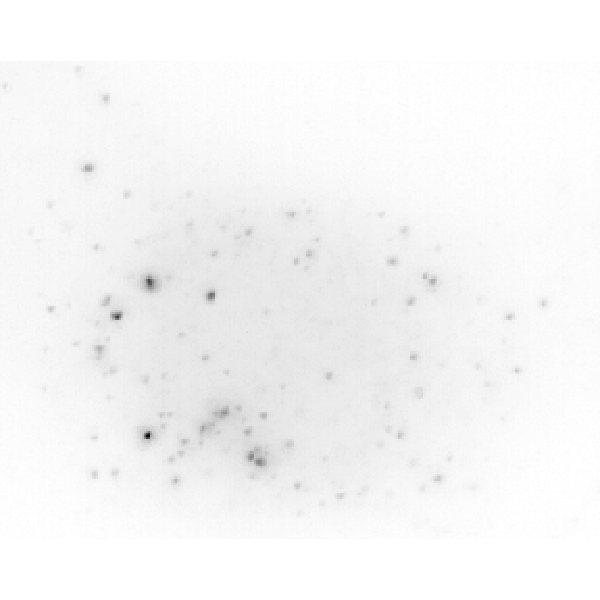
\includegraphics[width=0.95\linewidth]{figures/introduction/real_image_foci}
		\vfill
		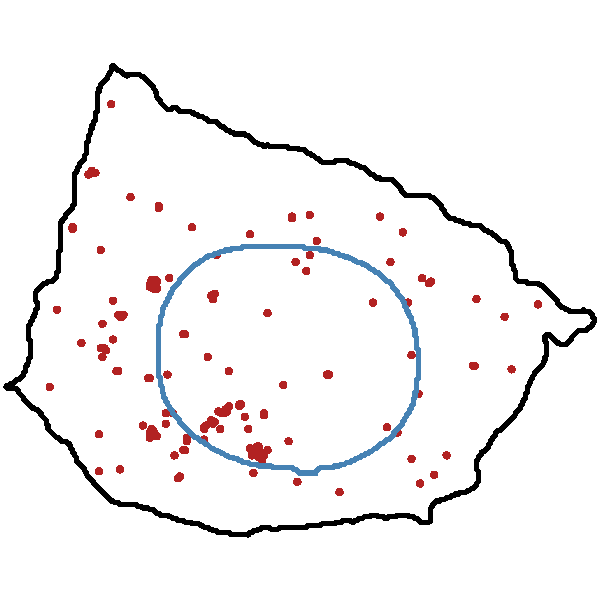
\includegraphics[width=0.95\linewidth]{figures/introduction/real_coord_foci}
		\subcaption{Foci}
	\endminipage\hfill
	\minipage{0.2\textwidth}
		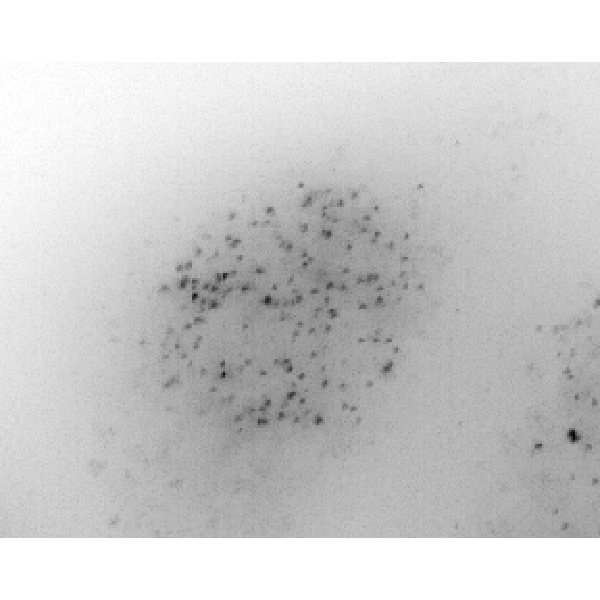
\includegraphics[width=0.95\linewidth]{figures/introduction/real_image_intranuclear}
		\vfill
		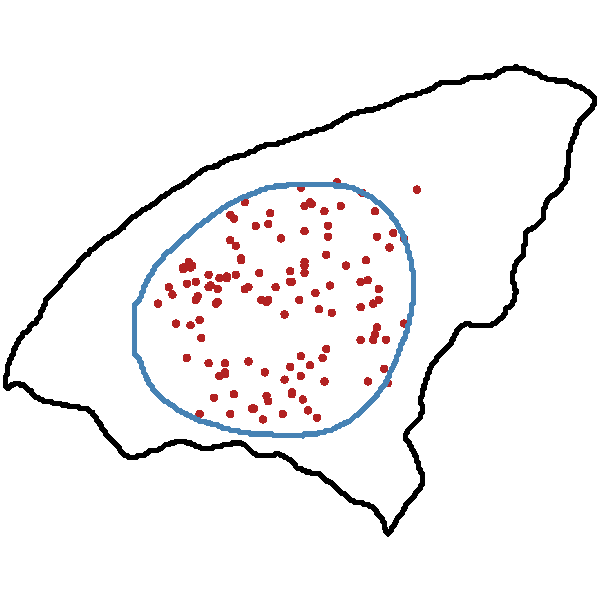
\includegraphics[width=0.95\linewidth]{figures/introduction/real_coord_intranuclear}
		\subcaption{Intranuclear}
	\endminipage\hfill
	\minipage{0.2\textwidth}
		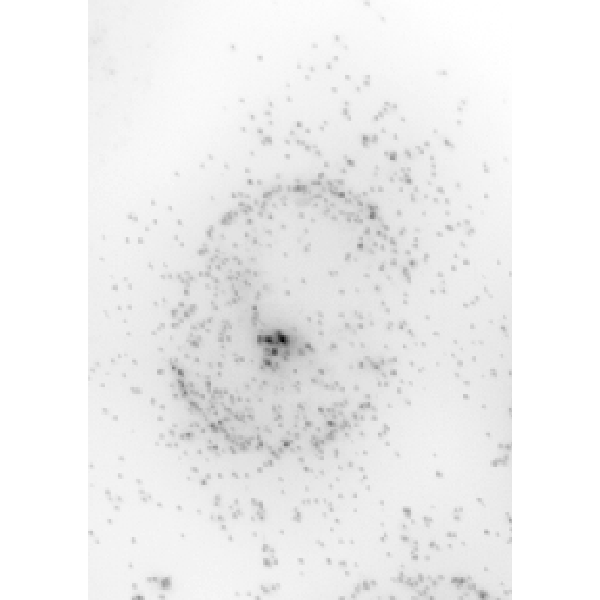
\includegraphics[width=0.95\linewidth]{figures/introduction/real_image_nuclear_edge}
		\vfill
		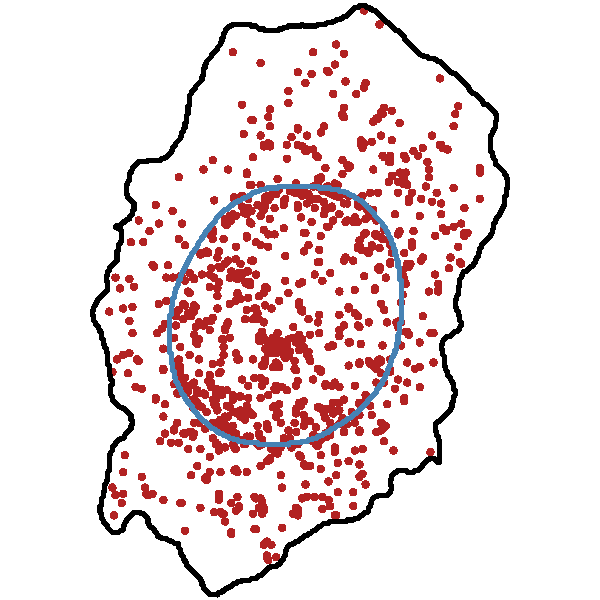
\includegraphics[width=0.95\linewidth]{figures/introduction/real_coord_nuclear_edge}
		\subcaption{Nuclear edge}
	\endminipage\hfill
	\minipage{0.2\textwidth}
		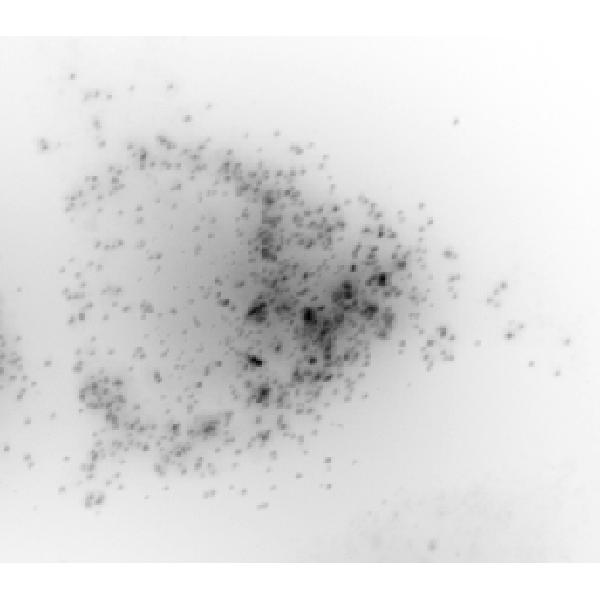
\includegraphics[width=0.95\linewidth]{figures/introduction/real_image_perinuclear}
		\vfill
		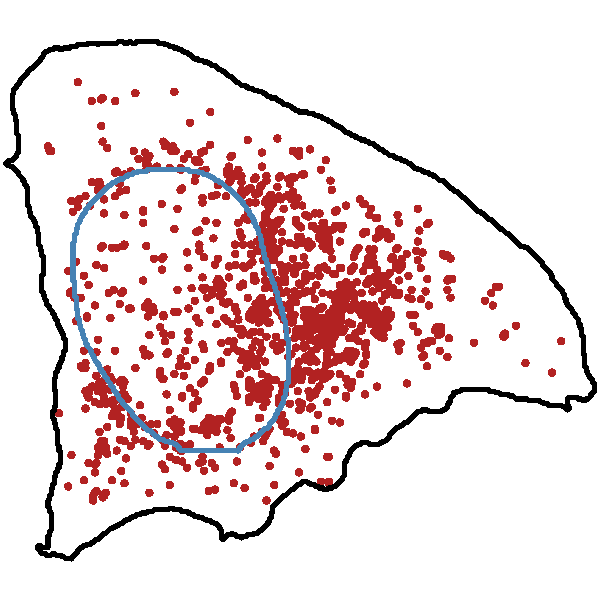
\includegraphics[width=0.95\linewidth]{figures/introduction/real_coord_perinuclear}
		\subcaption{Perinuclear}
	\endminipage\hfill
	\minipage{0.2\textwidth}
		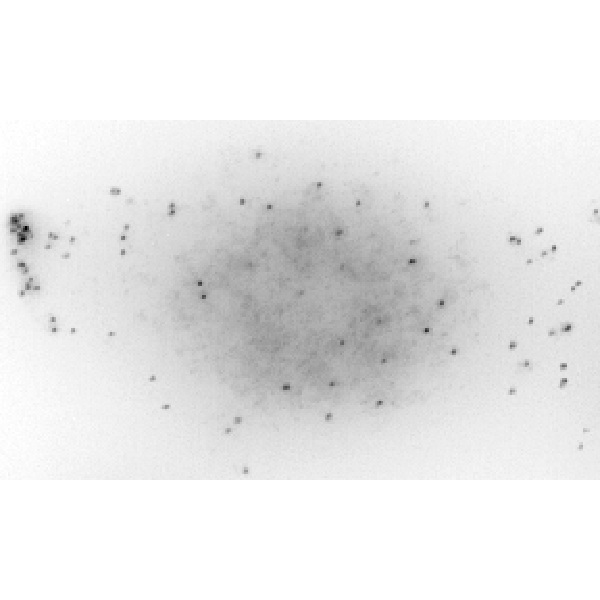
\includegraphics[width=0.95\linewidth]{figures/introduction/real_image_protrusion}
		\vfill
		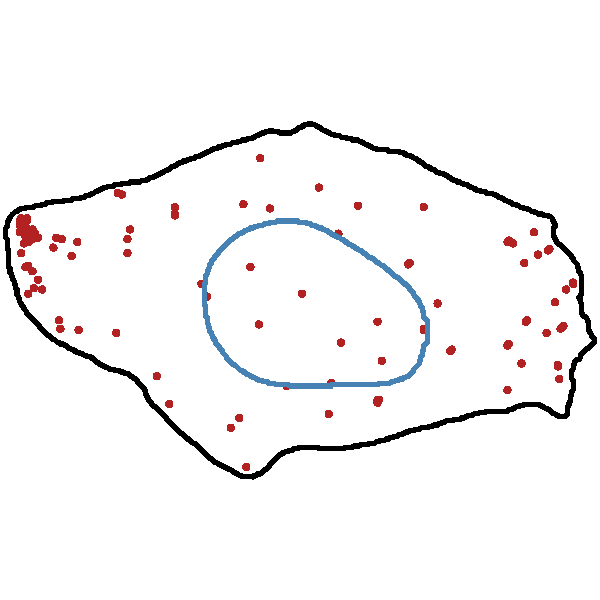
\includegraphics[width=0.95\linewidth]{figures/introduction/real_coord_protrusion}
		\subcaption{Protrusion}
	\endminipage
	\caption[RNA localization patterns: from pixels to numbers]{RNA localization patterns from~\cite{pointfish_2022}.
	(\textit{Top}) Typical smFISH images with different RNA localization patterns.
	(\textit{Bottom}) Coordinate representations with RNA spots (red), cell membrane (black) and nuclear membrane (blue).
	Detection and segmentation results are extracted and visualized with FISH-quant~\cite{Imbert_fq_2022}}
	\label{fig:intro_localization_patterns}
\end{figure}

\subsection{Bioinformatics in a nutshell}
\label{subsec:intro_non_ml_tools}

\subsection{A machine learning boom}
\label{subsec:intro_ml_tools}

%%%%%%%%%%%%%%%%%%%%%%%%%%%%%%%%%%%%%%%%%%%%%%%%%%%%%%%%%%%%%%%%%%%%%%%%%%%%%%%%%%%%%%%%%%%%%%%%%%%%%%%%%%%%%%%%%%%%%%%%%%%%%%%%%%%%%%%%%%%%%%%%%%%%%%%%%%%%
%%%%%%%%%%%%%%%%%%%%%%%%%%%%%%%%%%%%%%%%%%%%%%%%%%%%%%%%%%%%%%%%%%%%%%%%%%%%%%%%%%%%%%%%%%%%%%%%%%%%%%%%%%%%%%%%%%%%%%%%%%%%%%%%%%%%%%%%%%%%%%%%%%%%%%%%%%%%
%%%%%%%%%%%%%%%%%%%%%%%%%%%%%%%%%%%%%%%%%%%%%%%%%%%%%%%%%%%%%%%%%%%%%%%%%%%%%%%%%%%%%%%%%%%%%%%%%%%%%%%%%%%%%%%%%%%%%%%%%%%%%%%%%%%%%%%%%%%%%%%%%%%%%%%%%%%%

\section{Goals and contributions}
\label{sec:contributions}

\subsection{Goals}
\label{subsec:intro_goals}

At the beginning of my PhD, three main goals were defined with my supervisors.
The first one was the development and the implementation of a complete pipeline to process \ac{smFISH} images and return valuable insights about \ac{RNA} localization.
In particular, it was expected to integrate and adapt the latest successful developments in computer vision.
The second goal was the identification of bottlenecks that would prevent scaling the analysis to thousands images, in high content screening assays.
Such bottlenecks should be minimized or solved during the thesis to be able to scale any computational analysis based on \ac{smFISH} experiments.
Lastly, this complete framework would be applied to real experimental datasets in ongoing biological studies.

% add presentation of the localization patterns (from pixel to coord + patterns)
% mention Weeks et al. (1985) as firstpublication about RNA localization
% adham thesis: "Messenger localization was first discovered in Xenopus oocytes (Weeks et al., 1985)."

\subsection{Contributions}
\label{subsec:intro_contributions}

Beyond this own manuscript, my contributions are essentially lines of code.
With a effort of transparency, reproducibility and documentation, I try to develop computational tools as useful as possible for any biologist interested in \ac{FISH} experiments.
My PhD results in three major contributions.

\begin{itemize}
	\setlength\itemsep{0.1em}
	\item My first and main contribution is FISH-quant V2.
	This online framework gathers Python packages and a \ac{GUI} to process \ac{FISH} images, build robust analysis pipelines and even perform simulations.
	\item My second important contribution is an alternative method to compute relevant features in order to discriminate \ac{RNA} localization patterns.
	This method implies the development of PointFISH, a dedicated deep learning model for point cloud.
	\item My third contribution is my participation to biological studies with meaningful results.
	These studies leveraged high content screening assays and \ac{smFISH} techniques to perform a systemic analysis of \ac{RNA} localization and investigate local translation phenomenons.
\end{itemize}

\noindent
Some other contributions are also mentioned throughout this manuscript.
It includes a dataset I annotated for nucleus and cell segmentation with thousands of instances and my supervision of an intern.
The work performed during this internship was the seed for the first publication of another PhD student in the team, about in silico labeling and segmentation.
Lastly, a list of my publications are available at the very end of the manuscript.

\subsection{Manuscript summary}
\label{subsec:intro_manuscript}

The manuscript is composed of two parts.
The first four chapters are a presentation of the analysis pipeline with a focus on every critical stage.
It includes systematic reviews of the existing methods and details about solutions I implemented.
In addition, code snippets, ready to be imported and run, are interspersed with descriptions of the related algorithms.
The second part details several applications of my tools, where quantification of \ac{RNA} localization patterns supports biological insights.

In \textbf{Chapter~\ref{ch:chapter1}}, I present the general computational framework I developed and published: FISH-quant v2.
It includes methods for every stages of a \ac{FISH}-based analysis, with an effort to make them scalable and modular.
I also describe the improvements from the original FISH-quant version, and how it addresses the requirements of a modern software tool.

In \textbf{Chapter~\ref{ch:chapter2}}, I focus on the \ac{RNA} detection stage.
With \ac{smFISH} experiments, the \ac{RNA} molecules are spotted and reduced to discrete data points in space.
I describe detection algorithms and their extensions available in FISH-quant.
In the end, the set of all \ac{RNA} molecules is reduced to a point cloud with spatial coordinates.

In \textbf{Chapter~\ref{ch:chapter3}}, I review and describe algorithms for nucleus and cell segmentation.
Most of them are deep learning models, trained on vast datasets of annotated images.
Beside my own implemented methods, I also present refinement techniques to improve and format segmentation masks.
Two other projects for which I contributed (including one published) are also discussed at the end of the chapter.
They aim at improving the efficiency and consistency of segmentation on specific aspects.

In \textbf{Chapter~\ref{ch:chapter4}}, I compare two different approaches to quantify \ac{RNA} localization patterns.
Once the \ac{RNA} molecules are detected and cell morphology is segmented, the pixel domain gives way to Euclidean space and cells can be represented with a coordinate representation.
Then, spatial features are computed in order to discriminate relevant localization pattern.
I present two different methods of feature engineering.
The first method consists in manually designing features to characterize specific localization patterns.
I then list and describe every hand-crafted feature implemented in FISH-quant.
The second (published) method consists in learning features.
They are extracted from a deep learning model fed with the \ac{RNA} point cloud as input and trained on a simulated pretext task.

In \textbf{Chapter~\ref{ch:chapter5}}, I present several applications of my quantitative pipeline.
These applications come from three publications where we study different \ac{RNA} localization patterns and cases of local translation.
My analyses support and validates biological insights claimed in these studies about \ac{RNA} localization.
I design a classification pipeline to recognize generic localization patterns.
I evaluate the impact of translation inhibitor on \ac{RNA} localization and help identifying a singular translation-dependent pattern.
I quantify a cell cycle dependent pattern, which is related to centrosomes.
Finally, I also contribute to a a study focused on the protrusion pattern.

%%%%%%%%%%%%%%%%%%%%%%%%%%%%%%%%%%%%%%%%%%%%%%%%%%%%%%%%%%%%%%%%%%%%%%%%%%%%%%%%%%%%%%%%%%%%%%%%%%%%%%%%%%%%%%%%%%%%%%%%%%%%%%%%%%%%%%%%%%%%%%%%%%%%%%%%%%%%
%%%%%%%%%%%%%%%%%%%%%%%%%%%%%%%%%%%%%%%%%%%%%%%%%%%%%%%%%%%%%%%%%%%%%%%%%%%%%%%%%%%%%%%%%%%%%%%%%%%%%%%%%%%%%%%%%%%%%%%%%%%%%%%%%%%%%%%%%%%%%%%%%%%%%%%%%%%%
%%%%%%%%%%%%%%%%%%%%%%%%%%%%%%%%%%%%%%%%%%%%%%%%%%%%%%%%%%%%%%%%%%%%%%%%%%%%%%%%%%%%%%%%%%%%%%%%%%%%%%%%%%%%%%%%%%%%%%%%%%%%%%%%%%%%%%%%%%%%%%%%%%%%%%%%%%%%

% plots

% (RNA maturation)
% RNA transport mechanism

% smFISH + microscope
% multichannel images (dapi + smfish)
% multiplexed FISH

% (deep learning architecture)